\documentclass{scrartcl}
\usepackage[mathletters]{ucs}
\usepackage[utf8x]{inputenc}
\usepackage{amssymb}
\usepackage{amsmath}
\usepackage[usenames]{color}
\usepackage{hyperref}
\usepackage{wasysym}
\usepackage{graphicx}
\usepackage[normalem]{ulem}
\usepackage{enumerate}

\usepackage{listings}

\lstset{ %
basicstyle=\footnotesize,       % the size of the fonts that are used for the code
showspaces=false,               % show spaces adding particular underscores
showstringspaces=false,         % underline spaces within strings
showtabs=false,                 % show tabs within strings adding particular underscores
frame=single,                   % adds a frame around the code
tabsize=2,                      % sets default tabsize to 2 spaces
breaklines=true,                % sets automatic line breaking
breakatwhitespace=false,        % sets if automatic breaks should only happen at whitespace
}


\title{Masterproef Tool Wear Inspection - Update 3 TJ}
\date{dinsdag 08 december 2020}
\author{}

\begin{document}

\maketitle

		\section{Masterproef Tool Wear Inspection - Update 3 TJ}

Created vrijdag 20 november 2020



\subsection{Mail}



Best Tom,

 

Zoals aan het begin van de maand besproken zou ik graag afspreken om 200 nieuwe gelabelde plaatjes te komen ophalen.

Hierbij geef ik ook graag een update over mijn masterproef, waar ik sta en hoe de planning er op korte termijn uitziet.

 

Ik had even geleden nog een mail gestuurd met de vraag hoe de labels voor de plaatjes te onderscheiden zijn, wat is de A kant en wat is de B kant? Zou u hier kort op willen antwoorden gezien dit belangrijk is wanneer ik mijn foto’s ga testen.

 

Om de extra plaatjes te komen ophalen ben ik beschikbaar op volgende dagen steeds tussen 10:00 uur en 18:00 uur:

Maandag 02/11

Woensdag 04/11

Vrijdag 05/11

Woensdag 11/11

Vrijdag 13/11

 

Wanneer zou dit voor u passen?

 

Momenteel ben ik volop aan het werken aan een testopstelling die op een relatief snelle manier veel verschillende datasets kan genereren. Hierbij zijn een aantal belichtingsmogelijkheden en verschillen in camera posities die moeten kunnen getest worden op een heel aantal plaatjes om een resultaat te kunnen zien.

Om geautomatiseerd foto’s te kunnen nemen heb ik een rad ge-3D-print waarop de plaatjes kunnen worden vastgeklikt. Dit wordt dan aangestuurd met een stapmotor om 20 plaatjes in één batch te kunnen fotograferen. Zo kan de belichting en de camera vast blijven staan en zijn het de plaatjes die bewegen wat de hele opstelling vergemakkelijkt.

 

Vorige week heb ik ook een microscoopcamera ter beschikking gekregen en daar al wat beelden mee gemaakt. Hieronder/in bijlage zijn hiervan foto’s te zien. Op de eerste foto is een plaatje te zien met een grote slijtage, te tweede van een met zeer weinig slijtage. Hier is te zien dat met een juiste belichting de fout heel mooi naar voor komt. De resultaten van de software zullen nog even uitblijven gezien ik nu de eerste week wil focussen op de opstelling.



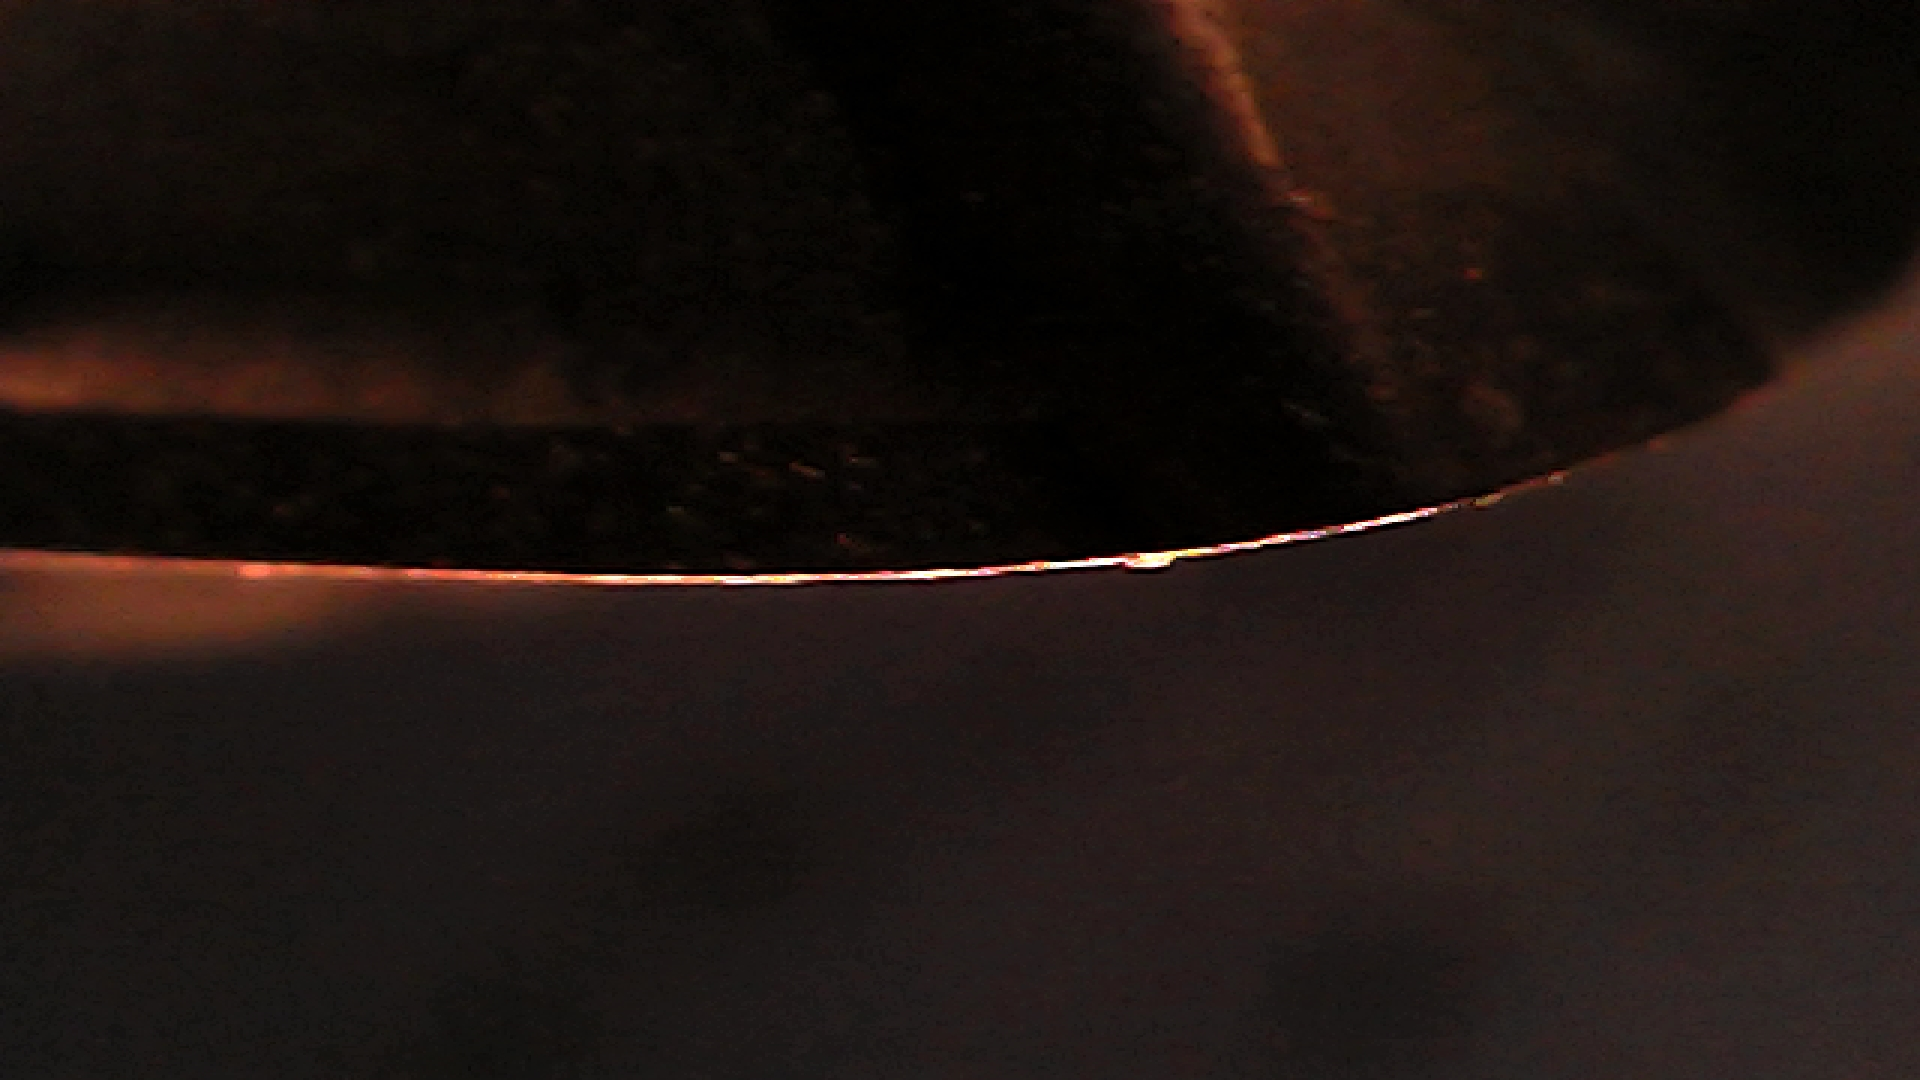
\includegraphics[width=4.166667in, keepaspectratio=true]{./Masterproef_Tool_Wear_Inspection_-_Update_3_TJ/eerste-opstelling_donkere_achtergrond3.jpg}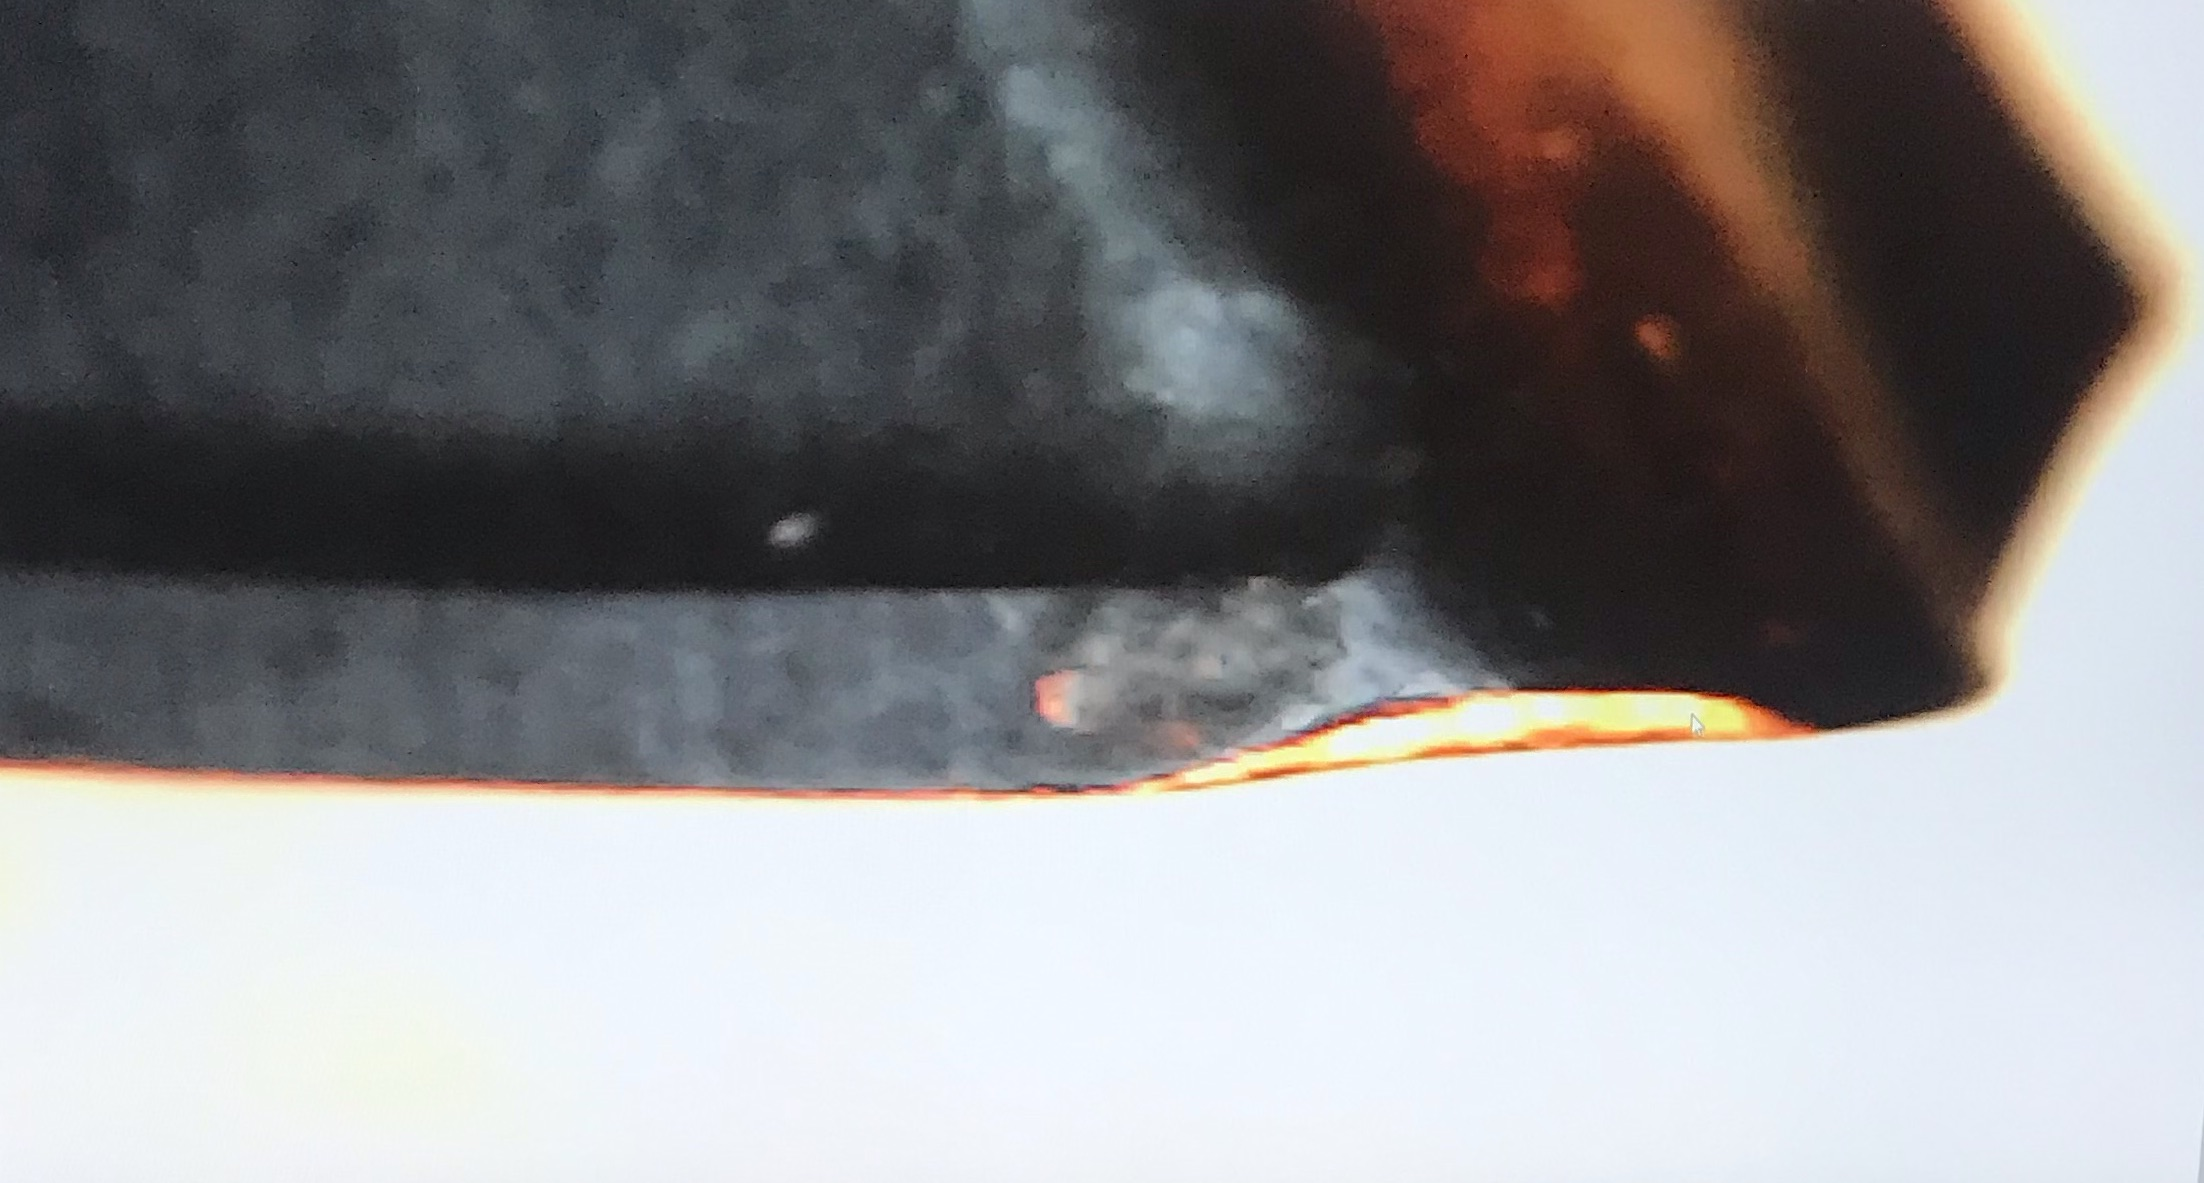
\includegraphics[width=4.166667in, keepaspectratio=true]{./Masterproef_Tool_Wear_Inspection_-_Update_3_TJ/eerste_setup_andere_richting_beeld2_screen image.jpeg}

 

Na de opstelling (binnen een goede week) begin ik aan een simpel algoritme dat zal bepalen of een plaatje goed of slecht is om met weinig foto’s te kunnen beslissen of een camera-opstelling goed is. Hierna kan ik met die opstelling de dataset verder uitbreiden en een algoritme maken en trainen om de effectieve fout te voorspellen in micron.

 

Met vriendelijke groeten,

 

Lars De Pauw



\end{document}
